\section{Type Analyzer}\label{sec:analyzer}

In this section, we explain the detail of the type analyzer of $\tool$. We first
formally define a modified $\ires$ and explain how to perform type analysis for
the modified $\ires$.  Moreover, we also explain a refinement of type analysis
based on conditions of assertions and branches to increase analysis precision.

\subsection{Intermediate Representation}\label{sec:ires}

$\ires$ is an untyped intermediate representation introduced by \citet{jiset}.
To make it more suitable for type analysis, we modify it as a label-based
language as follows:
\small
\[
  \begin{array}{l@{~}r@{~}c@{~}r@{~}r@{~}l}
    \text{Functions}
    &\funcset&\ni&\func&::=&\kwdef \; \x (\x^*, \x^*). \; \lab\\

    \text{Instructions}
    &\instset&\ni&\inst&::=&
    \kwlet \; \x = \expr \mid
    \kwlet \; \x = \kwrl \expr \; \expr^* \kwrr \mid
    \kwassert \; \expr \\

    &&&&\mid&
    \kwif \; \expr \; \lab \; \lab \mid
    \kwreturn \; \expr \mid
    \refer = \expr \\

    \text{References}
    &&&\refer&::=&
    \x \mid
    \refer \kwsl \expr \kwsr \\

    \text{Expressions}
    &&&\expr&::=&
    \tname \; \kwcl [\x: \expr]^* \kwcr \mid
    \clist{\expr^*} \mid
    \expr: \ty \mid
    \refer \kwexists \\

    &&&&\mid&
    \expr \bop \expr \mid
    \uop \; \expr \mid
    \refer \mid
    \const \mid
    \prim \\

    \text{Primitives}
    &\primset&\ni&\prim&::=&
    \undefval \mid \nullval \mid \bool \mid
    \num \mid \bigint \mid \str \mid \symb \\

    \text{Types}
    &\tyset&\ni&\ty&::=&\tname \mid \clist{} \mid \clist{\ty} \mid \tjs \mid
    \tprim \mid \undefval \mid \nullval\\

    &&&&\mid&
    \tbool \mid \tnumeric \mid \tnum \mid \tbigint \mid \tstr \mid \tsymb \\
  \end{array}
\]
A modified $\ires$ program $\prog = (\funcs, \getlab, \nextlab)$ is a triple of
a set of functions $\funcs \subseteq \and \funcset$ and two finite mappings
$\getlab$ and $nextlab$.  The getter mapping $\getlab: \labset \finmap \instset$
represents instructions attached to labels, and the next mapping $\nextlab:
\labset \finmap \labset$ denotes next labels.  A function $\kwdef \; \f (\x^*,
\y^*). \; \lab \in \funcset$ consists of a name $\f$, normal parameters $\x^*$,
optional parameters $\y^*$, and a body label $\lab$.  A label $\lab \in \labset$
denotes a program point.  An instruction $\inst$ is a variable declaration, a
function call, an assertion, a branch, a return, or an reference update.  Each
invocation of an abstract algorithm in ECMAScript is compiled to a function call
instruction with a newly introduced temporal variable.  We represent loops using
branch instructions with cyclic pointing of labels in the next mapping
$\nextlab$.  A reference $\refer$ is a variable $\x$ or a field access $\refer
\kwsl \expr \kwsr$.  An expression $\expr$ is a record, a list, a type check, an
existence check, a binary operation, a unary operation, a reference, a constant,
or a primitive, which is either $\undefval$, $\nullval$, a Boolean $\bool$, a
Number $\num$, a BigInt $\bigint$, a String $\str$, or a Symbol $\symb$.

\begin{figure}
  \centering
  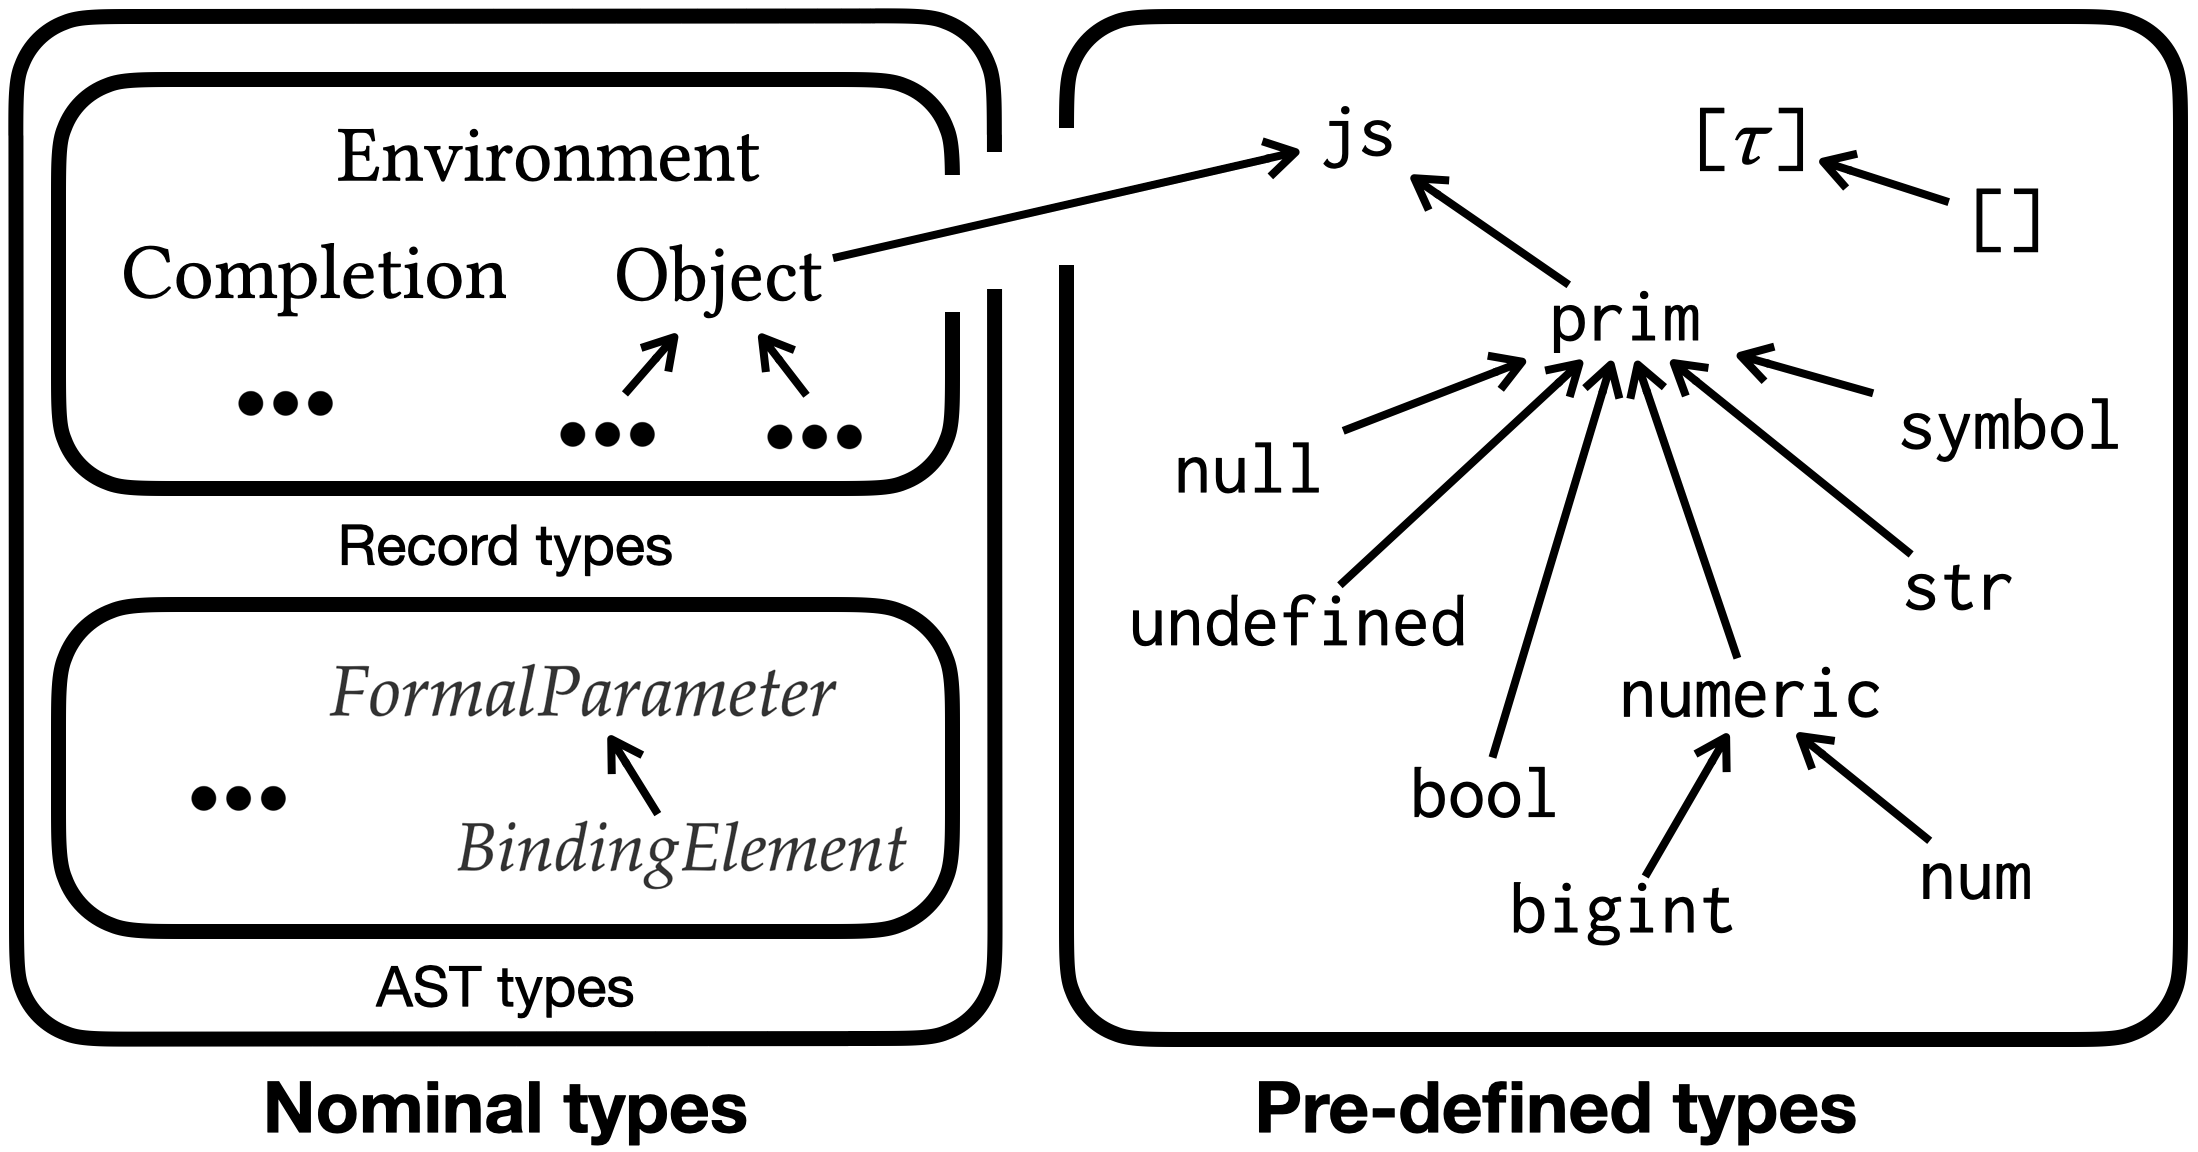
\includegraphics[width=0.48\textwidth]{img/subtype}
  \vspace*{-1.5em}
  \caption{A graphical representation of subtype relation $\subtype$.}
  \label{fig:subtype}
  \vspace*{-1.5em}
\end{figure}

A type $\ty \in \tyset$ is a norminal type $\tname$ or a pre-defined type;
$\tjs$ denotes JavaScript values, $\tprim$ primitives, $\tnumeric$ either Number
or BigInt values, and $\tnum$, $\tbigint$, $\tstr$, and $\tsymb$ denote Number,
BigInt, String, and Symbol values, respectively.  A norminal type $\tname$ is
either 1) a \textit{production type} for ASTs or 2) a \textit{record type} name
used in abstract algorithms, and ECMAScript describes its fields with
pre-defined or possible values.  A production type has corresponding
syntax-directed algorithms as its fields and a record type has specific fields
with possible values described in the corresponding table in ECMAScript.  For
example, the ``Table 10: References Record Fields'' in 
``Reference'' record has 

Each norminal type has own fields 
ECMAScript describes fields of each norminal type with their possible values in
table structures ad
scattered tables or syntax-directed algorithms
tables or 
It has pre-defined fields
It has fields

The subtype relation $\subtype \subseteq \tyset \times \tyset$ between types is
described in Figure~\ref{fig:subtype}; the directed edge from $\ty'$ to $\ty$
denotes $\ty' \subtype \ty$ and the relation is reflexive and transitive.  The
subtype relation is dependent on the syntax and defined record types in
ECMAScript.  We manually model subtypes between record types but automatically
extract subtypes for AST types.  For example, consider the syntax-directed
abstract algorithm at the right bottom in Figure~\ref{fig:example}.  The
non-terminal \textit{BindingElement} is the unique token in a alternative of
\textit{FormalParameter} thus we automatically extract the subtype relation:
\textit{BindingElement} $\subtype$ \textit{FormalParameter}.  Based on this
subtype relation, a type check expression $\expr: \ty$ checks whether the
evaluation result of $\expr$ has a type $\ty'$ satisfying $\ty' \subtype \ty$.
We represent semantics of the modified $\ires$ as a state transition system
$(\dom, \trans, \ielemset)$ with the transition relation $\trans \subseteq
\dom \times \dom$.  For presentation brevity, we omit its detail in this
paper and include it in a companion report~\inred{\cite{report}}.
% \[
%   \begin{array}{l@{~}r@{~}c@{~}r@{~}r@{~}l}
%     \text{States}
%     &\elem&\in&\dom&::=&\ctxtset^* \times \labset \times \envset\\
% 
%     \text{Contexts}
%     &\ctxt$\in$\ctxtset&::=&\labset \times \varset \times \envset\\
% 
%     \text{Environments}
%     &\env$\in$\envset&::=&\varset \finmap \valset\\
% 
%     \text{Values}
%     &\val$\in$\valset&::=& \addrset \uplus \addr \uplus \primset\\\
%   \end{array}
% \]


\subsection{Type Analysis}\label{sec:analysis}

We design a type analysis for the modified $\ires$ based on abstract
interpretation framework~\cite{ai1977, ai1992} with analysis
sensitivity~\cite{sens-toplas}.  We first extend types $\tyset$ to $\etyset$ as
follows:
\[
  \etyset \ni \ety ::=
  \ty \mid
  \func \mid
  \const \mid
  \tnormal(\ety) \mid
  \tabrupt \mid
  \bool \mid
  \str \mid
  \tabsent
\]
There are three different extensions; we add 1) functions and constants
because the original types $\tyset$ do not cover them, 2) normal completions
$\tnormal(\ety)$, abrupt completions $\tabrupt$, Boolean values $\bool$, and
String values $\str$ to increase the precision of type analysis. and 3) the
absent type $\tabsent$ to represent the existence of variables.  Using such
extended types, we define abstract states with flow-sensitivity and
type-sensitivity for parameters as follows:
\[
  \begin{array}{lr@{~}c@{~}c@{~}r@{~}l}
    \text{Abstract States}
    &\aelem&\in&\adom&=&
    \viewset \rightarrow (\aenvset \times \partsof{\viewset})\\

    \text{Views}
    &\view&\in&\viewset&=&
    (\labset \times \etyset^*) \uplus
    (\funcset \times \etyset^*)\\

    \text{Abstract Environments}
    &\aenv&\in&\aenvset&=&\varset \rightarrow \atyset\\

    \text{Abstract Types}
    &\aty&\in&\atyset&=&\partsof{\etyset}\\
  \end{array}
\]
An abstract state $\aelem \in \adom$ is a mapping from views to pairs of
abstract environments and next views.  A view $\view$ is a pair of a label for
the flow-sensitivity and a
sequence of extended types for the type-sensitivity for parameters.  An abstract
environment $\aenv \in \aenvset$ is a mapping from variables to abstract types
and an abstract type is a set of extended types.


\begin{figure*}[t]
  \centering
  \begin{subfigure}[b]{0.48\textwidth}
    \[
      \begin{array}{r@{~}c@{~}l}
        \asem{\kwlet \; \x = \expr}
        ((\lab, \overline{\ety}), \aenv)(\aelem)
        &=& \todo \\

        \asem{\kwlet \; \x = \kwrl \expr_0 \; \expr_1 \cdots \expr_n \kwrr}
        ((\lab, \overline{\ety}), \aenv)(\aelem)
        &=& \todo \\

        \asem{\kwassert \; \expr}
        ((\lab, \overline{\ety}), \aenv)(\aelem)
        &=& \todo \\

        \asem{\kwif \; \expr \; \lab_0 \; \lab_1}
        ((\lab, \overline{\ety}), \aenv)(\aelem)
        &=& \todo \\

        \asem{\kwreturn \; \expr}
        ((\lab, \overline{\ety}), \aenv)(\aelem)
        &=& \todo \\

        \asem{\refer = \expr}
        ((\lab, \overline{\ety}), \aenv)(\aelem)
        &=& \todo \\
      \end{array}
    \]
    \caption{Instructions with $\asem{\inst}: (\viewset \times
    \aenvset) \rightarrow \adom \rightarrow \adom$}
  \end{subfigure}
  \begin{subfigure}[b]{0.48\textwidth}
    \[
      \begin{array}{r@{~}c@{~}l}
        \tname^? \; \kwcl [\x: \expr]^* \kwcr
        \clist{\expr^*}
        \expr: \ty
        \refer \kwexists
        \expr \bop \expr
        \uop \; \expr
        \refer
        \const
        \prim
      \end{array}
    \]
    \caption{Expressions with $\asem{\expr}: (\viewset \times \aenvset)
    \rightarrow \atyset$}
  \end{subfigure}
  \caption{Abstract semantics of $\ires$ components.}
  \label{fig:example}
\end{figure*}



\subsection{Refinement}\label{sec:refine}
